\documentclass[border=10pt]{standalone}
\usepackage{tikz}\usepackage{amsmath}\usetikzlibrary{calc,arrows.meta,decorations.markings}
\begin{document}
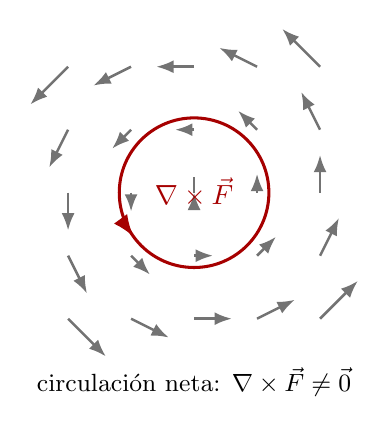
\begin{tikzpicture}[line width=0.9pt,>={Latex[length=2.2mm]}]
  % campo que circula
  \foreach \x in {-1.6,-0.8,0,0.8,1.6} \foreach \y in {-1.6,-0.8,0,0.8,1.6}{
    \pgfmathsetmacro{\ux}{-\y*0.30}\pgfmathsetmacro{\uy}{\x*0.30}
    \draw[->,black!55] (\x,\y)--++(\ux,\uy);
  }
  % lazo de circulacion
  \draw[->,red!65!black,line width=1.1pt,decoration={markings,mark=at position 0.6 with {\arrow{Latex}}},postaction={decorate}] (0,0) circle(0.95);
  \node[red!65!black] at (0,0){$\nabla\times\vec F$};
  \node at (0,-2.4){\small circulación neta: $\nabla\times\vec F\neq\vec 0$};
\end{tikzpicture}
\end{document}
